\documentclass{beamer}
\usepackage{graphicx}
\usepackage{amsmath}
\usepackage{kpfonts}
\usepackage{tikz}
\usepackage{setspace}

\usepackage{tikz}
\usetikzlibrary{shapes.geometric,arrows}
\tikzset{
	basics/.style={minimum width=30mm, minimum height=7.5mm, text centered, draw=black},
	startstop/.style={rectangle, rounded corners, basics, fill=red!30},
	io/.style={trapezium, trapezium left angle=70, trapezium right angle=110, basics, fill=blue!30},
	process/.style={rectangle, basics, fill=blue!30},
	decision/.style={ellipse,basics, fill=green!30},
	arrow/.style={thick,->,>=stealth},
}

%\usepackage{unicode-math}
%\usepackage{enumitem}
\usepackage{boxedminipage}
\newcommand\answerbox{%%
    \fbox{\rule{1in}{0pt}\rule[-0.5ex]{0pt}{4ex}}}
\usetheme{Warsaw}
\tikzset{>=latex}
\newcommand\stretchon{%
	\newpar%
	\renewcommand\item[1][\itemsymbol]{\svitem[##1]\newitem}%
	\renewenvironment{itemize}%
	{\svitemize}{\svenditemize\newpar\par}%
	\renewenvironment{center}%
	{\svcenter\newpar}{\svendcenter\newpar}%
	\renewenvironment{column}[2]%
	{\svcolumn{##1}\setlength{\parskip}{\columnskip}##2}%
	{\svendcolumn\vspace{\columnskip}}%
}
%%%%%%%%%%%%%%%%Title Page%%%%%%%%%%%%%%%%%%%%%%%%%%%%%%%%%

\title[SSL Project]{Form and survey management}
\subtitle[]{SSL Project}
\author[Dark Prince]{\textsc{\huge Team Dark Prince}}
\institute[IITB]{
  Department of Computer Science and Engineering\\
  IIT Bombay.\\
  Powai, Mumbai - 400076\\[1ex]
}
\date[\today]{\today}

%%%%%%%%%%%%%%%%%%%%%%%%%%%%%%%%%%%%%%%%%%%%%%%%%%%%%%%%%%%
\newtheorem{exercise}{Exercise}
\begin{document}
%--- the titlepage frame -------------------------%
\begin{frame}[plain]
  \titlepage 
\end{frame}

%%%%%%%%%%%%%%%%%%%%%%%%%%%%%%%%%%%%%%%%%%%%%%%%%%%%%%%%%%%
\begin{frame}
	\frametitle{Introduction}
	Our form and survey management tool lets you create your own completely modular forms, which can be shared with other users, and the data acquired with the forms can be analyzed in various ways like pie charts and bar graphs.
	\vspace{10pt}
	\begin{enumerate}
		\item \textbf{Features implemented}
		\begin{itemize}
			\item User authentication.
			\item Terminal Client.
		\end{itemize}
	\item \textbf{Tools used}
	\begin{itemize}
		\item \href{https://www.djangoproject.com/}{Django} for backend.
	\end{itemize}
	\end{enumerate}
\end{frame}
\begin{frame}
	\frametitle{Implementation Details}
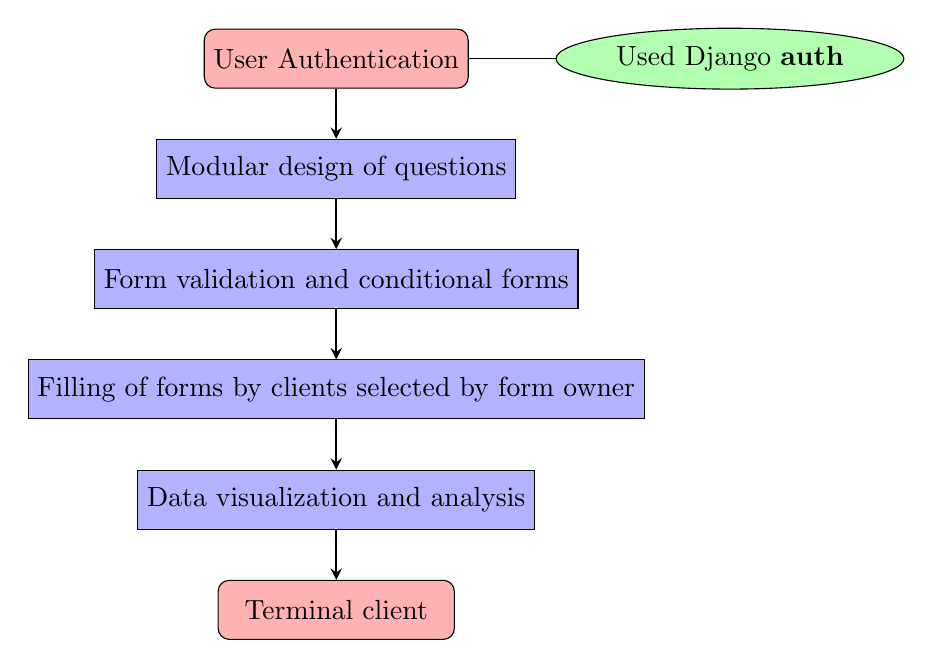
\begin{tikzpicture}[node distance=14mm]
\node (start) [startstop] {User Authentication};
\node (how) [decision,right of=start, node distance=50mm] {Used Django \textbf{auth}};
\node (in1) [process, below of=start] {Modular design of questions};
\node (out1) [process, below of=in1] {Form validation and conditional forms};
\node (out2) [process, below of=out1] {Filling of forms by clients selected by form owner};
\node (out3) [process, below of=out2] {Data visualization and analysis};
\node (out4) [startstop, below of=out3] {Terminal client};
\foreach \i/\j/\k in {start/in1/,in1/out1/,out1/out2/,out2/out3/,out3/out4/}
\draw [arrow] (\i) -- node[anchor=east] {\k} (\j);
\draw [-] (start) -- (how);
%\draw [arrow] (in1.east) -- +(20pt,0) |- (start.east) node [pos=.25, right] {No};
\end{tikzpicture}
\end{frame}
\begin{frame}
	\frametitle{Future plan of action}
	We will complete features in the following order
	\begin{enumerate}
		\item Modular design of questions
		\begin{itemize}
			\item November 15
			%\item Not yet decided
		\end{itemize}
	\item Form validation and conditional forms
	\begin{itemize}
		\item November 16
		%\item Not yet decided
	\end{itemize}
\item Data visualization and analysis
\begin{itemize}
	\item November 17
	\item We will be using \href{https://developers.google.com/chart}{\textbf{Google charts}} for this beacuse google charts are free and support cross-browser compatibility and cross platform portability.
\end{itemize}
	\end{enumerate}
\end{frame}
\begin{frame}
	\frametitle{Styling}
	\framesubtitle{An additional feature}
	We will give options for users to change theme and font style and we will change colors, font sizes using class selectors, CSS and bootstrap.
\end{frame}
\end{document}
